%
% vektorgeometrie.tex
%
% (c) 2018 Prof Dr Andreas Müller, Hochschule Rapperswil
%
\section{Vektorgeometrische Interpretation}
\rhead{Vektorschreibweise}
Die bisherigen rein algebraischen Betrachtungen verdecken den geometrischen
Gehalt der bisher entwickelten Theorie.
In diesem Abschnitt soll daher zunächst eine vektorielle Darstellung
aufgebaut werden, die dann erlauben soll, einerseits die Formeln für die 
Fourierkoeffizienten geometrisch zu verstehen und andererseits auf
komplexere Situationen zu verallgemeinern.

\subsection{Vektoren}
Die Operationen zur Bestimmung der Fourier-Koeffizienten können in 
vektorieller Schreibweise etwas übersichtlicher dargestellt werden.
Zunächst fassen wir die Funktionswerte $y_j$ in einem Vektor
\begin{equation}
y = \begin{pmatrix}y_1\\\vdots\\y_N\end{pmatrix}
\end{equation}
zusammen.
Zur Berechnung der Fourier-Koeffizienten brauchen wir auch noch die
Werte der trigonometrischen Funktionen zu den Zeiten $t_j$, die wir
ebenfalls als Vektoren
\begin{align*}
c_0&=\begin{pmatrix}1\\\vdots\\1\end{pmatrix},
&
c_k&=\begin{pmatrix}\cos kt_1\\\vdots\\\cos kt_N\end{pmatrix},\;(k=1,\dots,n)
&&\text{und}
&
s_k&=\begin{pmatrix}\sin kt_1\\\vdots\\\sin kt_N\end{pmatrix},\;(k=1,\dots,n-1)
\end{align*}
schreiben.

\subsubsection{Skalarprodukt und Norm}
Die Fourier-Koeffizienten sind Summen von Produkten von Komponenten von $y$
und Werten von trigonometrischen Funktionen, die wir ebenfalls als Komponenten
der Vektoren $c_k$ und $s_k$ ansehen können.
Dies sieht aus wie das Skalarprodukt zweier Vektoren.

Wir verwenden die folgende Notation.
Das Skalarprodukt zweier Vektoren $x$ mit Komponenten $x_j$ und $y$ mit
\index{Skalarprodukt}%
Komponenten $y_j$ ist
\begin{equation}
x\cdot y
=
\sum_{j=1}^N x_jy_j
=
x^ty.
\end{equation}
Die Norm eines Vektors ist
\index{Norm}%
\begin{equation}
\| x\| = \!\sqrt{x\cdot x} = \!\sqrt{\sum_{j=1}^N x_j^2}.
\end{equation}
Die Entfernung zwischen zwei Vektoren ist dann $\| x-y\|$.
Die Fourier-Analyse löst das Problem, Koeffzienten $a_k$ und $b_k$
zu finden, so dass der Vektor $y$ der Funktionswerte $y_j$ und
der Vektor $p_n$ der Werte $p_n(t_j)$ des trigonometrischen Polynoms
möglichst nahe beieinander sind.
Genauer wurde 
\begin{equation}
L=L(a_0,a_1,\dots,a_n,b_1,\dots,b_{n-1})
=
\sum_{j=1}^N (y_j - p_n(t_j))^2
=
\| y - p_n\|^2
\qquad\text{mit}\quad
p_n=\begin{pmatrix}
p_n(t_1)\\\vdots\\p_n(t_N)
\end{pmatrix}
\end{equation}
als zu minimierendes Mass für den Abstand der beiden Vektoren
definiert.

Die Fourier-Koeffizienten können jetzt als Skalarprodukte geschrieben werden:
\begin{align*}
a_0
&=
\frac1N\sum_{j=1}^N y_j
=
\frac1N\sum_{j=1}^N 1\cdot y_j 
=
\frac1N c_0\cdot y,
\\
a_k
&=
\frac{2}{N}\sum_{j=1}^N
\cos kt_j \cdot y_j
=
\frac2N c_k\cdot y,
&k&=1,\dots n
\\
b_k
&=
\frac2N \sum_{j=1}^N \sin kt_j \cdot y_j
=
\frac2N s_k\cdot y,&k&=1,\dots,n-1
\end{align*}

\subsubsection{Rekonstruktion der Funktion}
Auch die Darstellung der Funktion kann man wieder als Skalarprodukt schreiben.
Dazu schreiben wir die Fourier-Koeffizienten und die Werte der
trigonometrischen Funktionen also Vektoren
\[
\begin{aligned}
a
&=
\begin{pmatrix}
a_0\mathstrut\\
a_1\mathstrut\\
b_1\mathstrut\\
a_2\mathstrut\\
b_2\mathstrut\\
\vdots\\
b_{n-1}\mathstrut\\
a_n\mathstrut
\end{pmatrix}
&&\text{und}
&
e(t)
&=
\begin{pmatrix}
1\\
\cos t\\
\sin t\\
\cos2t\\
\sin2t\\
\vdots\\
\sin(n-1)t\\
\cos nt
\end{pmatrix}.
\end{aligned}
\]
Damit wird 
\begin{align*}
p_n(t)
&=
a_0 + a_1\cos t + b_1\sin t + a_2\cos2t+b_2\sin2t+\dots+a_n\cos nt
\\
&=
\begin{pmatrix}
a_0\mathstrut\\
a_1\mathstrut\\
b_1\mathstrut\\
a_2\mathstrut\\
b_2\mathstrut\\
\vdots\\
b_{n-1}\mathstrut\\
a_n\mathstrut
\end{pmatrix}
\cdot
\begin{pmatrix}
1\\
\cos t\\
\sin t\\
\cos2t\\
\sin2t\\
\vdots\\
\sin(n-1)t\\
\cos nt
\end{pmatrix}
=
a\cdot e(t).
\end{align*}
Der Vektor $p_n$ besteht aus Funktionswerten $p_n(t_j)$, man kann dies
auch als Linearkombination der Vektoren $c_0$, $c_k$ und $s_k$ schreiben:
\begin{equation}
p_n = a_0c_0 + \sum_{k=1}^n a_kc_k + \sum_{k=1}^{n-1} b_ks_k.
\label{skript:fourier:pn}
\end{equation}

\subsubsection{Gleichungen für die Koeffizienten}
Sogar die Herleitung der Gleichungen zur Bestimmung der Fourierkoeffizienten
lässt sich in dieser vektoriellen Schreibweise kompakter durchführen.
Die Ableitung von $L$ nach einem Koeffizienten ist
\begin{align*}
\frac{\partial L}{\partial a_0}
&=
\frac{\partial}{\partial a_0} (y-p_n)\cdot (y-p_n)
=
-2(y-p_n)\cdot \frac{\partial p_n}{\partial a_0}
\\
\frac{\partial L}{\partial a_k}
&=
\frac{\partial}{\partial a_k} (y-p_n)\cdot (y-p_n)
=
-2(y-p_n)\cdot \frac{\partial p_n}{\partial a_k}
\\
\frac{\partial L}{\partial b_k}
&=
\frac{\partial}{\partial b_k} (y-p_n)\cdot (y-p_n)
=
-2(y-p_n)\cdot \frac{\partial p_n}{\partial b_k}.
\end{align*}
Die Ableitungen des Vektors $p_n$ nach den Koeffizienten sind
\begin{align*}
\frac{\partial p_n}{\partial a_0}
&=
\begin{pmatrix}
1\\
\vdots\\
1
\end{pmatrix}
=
c_0,&
\frac{\partial p_n}{\partial a_k}
&=
\begin{pmatrix}
\cos kt_1\\\vdots\\\cos kt_N
\end{pmatrix} = c_k,
&
\frac{\partial p_n}{\partial b_k}
&=
\begin{pmatrix}
\sin kt_j\\\vdots\\\sin kt_N,
\end{pmatrix}
\end{align*}
womit die Gleichungen zur Bestimmung der Fourierkoeffizienten zu
\begin{align*}
(y-p_n)\cdot c_0 &= 0&
(y-p_n)\cdot c_k &= 0&
(y-p_n)\cdot s_k &= 0
\end{align*}
werden.
Die Darstellung~\eqref{skript:fourier:pn} des Vektors $p_n$ erlaubt,
diese Gleichungen weiter zu vereinfachen, sie werden zu
\begin{equation}
\begin{aligned}
(y-p_n)\cdot c_0&=0 
&&\Rightarrow&
y\cdot c_0
&=
\biggl(a_0c_0 + \sum_{k=1}^n a_kc_k +\sum_{k=1}^{n-1}b_ks_k\biggr)\cdot c_0
\\
(y-p_n)\cdot c_k&=0 
&&\Rightarrow&
y\cdot c_k
&=
\biggl(a_0c_0 + \sum_{k=1}^n a_kc_k +\sum_{k=1}^{n-1}b_ks_k\biggr)\cdot c_k
\\
(y-p_n)\cdot s_k&=0 
&&\Rightarrow&
y\cdot s_k
&=
\biggl(a_0c_0 + \sum_{k=1}^n a_kc_k +\sum_{k=1}^{n-1}b_ks_k\biggr)\cdot s_k
\end{aligned}
\label{skript:fourier:skalarprodgl}
\end{equation}
Die Summen auf der rechten Seite können ausgewertet werden, wenn man
die Skalarprodukte der Vektoren $c_k$ und $s_k$ kennt.

\subsubsection{Orthogonalität}
Die Aussagen von Satz~\ref{skript:fourier:orthogonalitaet1}
lassen sich jetzt in geometrische Form fassen.
\begin{satz}
Es gilt
\begin{align*}
c_k\cdot c_l
&=
\begin{cases}
N&\qquad k=l=0\\
\displaystyle\frac{N}2&\qquad k=l>0\\
0&\qquad\text{sonst}
\end{cases}
\\
s_k\cdot s_l
&=
\begin{cases}
\displaystyle\frac{N}2&\qquad k=l\\
0&\qquad\text{sonst}
\end{cases}
\\
c_k\cdot s_l
&=
0
\end{align*}
\label{skript:fourier:orthogonalitaet}
\end{satz}

\begin{proof}[Beweis]
Die genannten Skalarprodukte sind nichts anderes als die Summen in
Satz~\ref{skript:fourier:orthogonalitaet1}:
\begin{align*}
c_k\cdot c_l
&=
\sum_{j=1}^N \cos kt_j \cos lt_j
=
\begin{cases}
N&\qquad k=l=0\\
\displaystyle\frac{N}2&\qquad k=l>0\\
0&\qquad\text{sonst}
\end{cases}
\end{align*}
und analog für die anderen Skalarprodukte.
Die Aussage des Satzes~\ref{skript:fourier:orthogonalitaet}
ist daher nichts anders als eine geometrische
Umformulierung der Aussagen des
Satzes~\ref{skript:fourier:orthogonalitaet1}.
\end{proof}

In den Gleichungen~\eqref{skript:fourier:skalarprodgl} können jetzt
die Skalarprodukte berechnet werden.
Es bleibt jeweils nur ein einziger Term übrig, nämlich
\begin{equation*}
\begin{aligned}
y\cdot c_0 &= a_0 c_0\cdot c_0
&&\Rightarrow&
a_0 = \frac{1}{c_0\cdot c_0}c_0\cdot y = \frac1N c_0\cdot y
\\
y\cdot c_k &= a_k c_k\cdot c_k
&&\Rightarrow&
a_k = \frac{1}{c_k\cdot c_k}c_k\cdot y = \frac2N c_k\cdot y
\\
y\cdot s_k &= b_k s_k\cdot s_k
&&\Rightarrow&
b_k = \frac{1}{s_k\cdot s_k}s_k\cdot y = \frac2N s_k\cdot y,
\end{aligned}
\end{equation*}
wie früher auch schon gefunden.

\subsubsection{Die Identität von Parseval}
Die Relationen von
Satz~\ref{skript:fourier:orthogonalitaet1}
besagen, dass die Vektoren $c_k$ und $s_k$ orthogonal sind.
Wir wenden Sie auf das Skalarprodukt der Funktion $f$ mit sich selbst an.
\begin{align*}
f\cdot f
&=
a_0^2 c_0\,\cdot c_0
+
\sum_{k=1}^na_k^2 \,c_k\cdot c_k
+
\sum_{k=1}^{n-1} b_k^2\,s_k\cdot s_k
\\
&=
Na_0^2
+
\frac{N}2\sum_{k=1}^n a_k^2
+
\frac{N}2\sum_{k=1}^{n-1} b_k^2
=
\frac{N}2
\biggl(
2a_0^2
+
\sum_{k=1}^n a_k^2
+
\sum_{k=1}^{n-1} b_k^2
\biggr).
\end{align*}
Damit haben wir den folgenden Satz bewiesen:
\begin{satz}[Parseval]
\[
\|f\|^2
=
\sum_{j=1}^N y_j^2
=
\frac{N}2
\biggl(
2a_0^2
+
\sum_{k=1}^n a_k^2
+
\sum_{k=1}^{n-1} b_k^2
\biggr).
\]
\end{satz}
\index{Parseval-Gleichung}%
Die Parseval-Gleichung hat zur Konsequenz, dass eine Funktion mit nur
kleinen Werten auch nur kleine Fourier-Koeffizienten haben kann.
Sind zwei Funktionen $f$ und $g$ nahe beieinander, dann unterscheiden
sich die Fourier-Koeffizienten nur wenig.

Umgekehrt können wir auch schliessen, dass Terme mit kleinen
Fourier-Koeffizienten nur zu geringen Unterschieden der Funktionen
führen.
Indem wir Terme mit kleinen Fourier-Koeffizienten weglassen, 
können wir die Approximation einer Funktion durch ein trigonometrisches
Polynom vereinfachen, ohne dass ein grosser Fehler entsteht.

\subsection{$2\pi$-periodische Funktionen auf $\mathbb R$\label{subsection:fourier:stetig}}
Die eben vektoriell dargestellte Analyse diskreter periodischer Funktionen 
kann verallgemeinert werden auf die Analyse von Funktionen auf
anderen Definitionsgebieten.
Benötigt wird eine Familie von Basisfunktionen und ein Skalarprodukt
$\langle\;,\;\rangle$ derart, dass die Basisfunktionen $g_i$ bezüglich
dieses Skalarproduktes orthonormiert sind, dass also
\[
\langle g_i,g_j\rangle
=
\delta_{ij}
=
\begin{cases}
1&\qquad i=j\\
0&\qquad\text{sonst}.
\end{cases}
\]
Jede Linearkombination
\[
f = \sum_{i} \alpha_i g_i
\]
von Basisfunktionen kann ebenfalls mit dem Skalarprodukt rekonstruiert
werden.
Dazu berechnet man
\[
\langle g_i,f\rangle
=
\biggl\langle
g_i,\sum_j\alpha_jg_j
\biggr\rangle
=
\sum_j \langle g_i,\alpha_jg_j\rangle
=
\sum_j \alpha_j\delta_{ij}
=
\alpha_i.
\]
Das Skalarprodukt kann auch verwendet werden, um einen Abstand zwischen
Vektoren als
\[
\| f-g\|^2
=
\langle f-g,f-g\rangle
\]
zu definieren.

Dieselbe Situation lässt sich auch für $2\pi$-periodische Funktionen 
auf $\mathbb R$ herbeiführen.
Als Basisfunktionen kann man die Funktionen 
\begin{equation}
\frac{1}{\!\sqrt{2}},\; \cos kx,\; \sin lx\quad k>0
\label{fourier:basis}
\end{equation}
verwenden.
Das Skalarprodukt $\langle f,g\rangle$ muss linear in $f$ und $g$ sein.
Eine nahe liegende Wahl dafür ist
\[
\langle f, g\rangle
=
\frac{1}{\pi}\int_{-\pi}^{\pi} f(x)\,g(x)\,dx.
\]
Wir überprüfen, ob die Funktionen orthogonal sind:
\begin{align*}
\left\langle \frac1{\!\sqrt{2}},\frac1{\!\sqrt{2}}\right\rangle
&=
\frac1{\pi}
\int_{-\pi}^{\pi} \frac12\,dx
=
1
\\
\left\langle \frac1{\!\sqrt{2}},\cos kx\right\rangle
&=
\frac1{\pi}\int_{-\pi}^{\pi}
\frac1{\!\sqrt{2}}\cos kx
\,dx
=0
\\
\left\langle \frac1{\!\sqrt{2}},\sin kx\right\rangle
&=
\frac1{\pi}\int_{-\pi}^{\pi}
\frac1{\!\sqrt{2}}\sin kx
\,dx
=0
\\
\langle \cos kx,\cos lx\rangle
&=
\frac1{\pi}
\int_{-\pi}^\pi \cos kx\cos lx\,dx
\\
&=
\frac1{\pi}
\int_{-\pi}^\pi
\frac12\bigl(
\cos (k-l)x+\cos (k+l)x
\bigr)
\,dx
=
\begin{cases}
1&\qquad k=l\\
0&\qquad\text{sonst}
\end{cases}
\\
\langle \sin kx,\sin lx\rangle
&=
\frac1{\pi}
\int_{-\pi}^\pi \sin kx\,\sin lx\,dx
\\
&=
\frac1{\pi}
\int_{-\pi}^\pi
\frac12
\bigl(
\cos (k-l)x - \cos (k+l)x
\bigr)
\,dx
=
\begin{cases}
1&\qquad k=l\\
0&\qquad\text{sonst}
\end{cases}
\\
\langle \sin kx,\cos lx\rangle
&=
\frac1{\pi}
\int_{-\pi}^{\pi} 
\frac12\bigl(
\sin (k-l)x + \sin (k+l)x
\bigr)
\,dx
=0
\end{align*}
Zu einer $2\pi$-periodischen Funktion $f(x)$ kann man daher immer
die Koeffizienten
\begin{equation}
\begin{aligned}
\bar{a}_0&=\frac1{\pi\!\sqrt{2}}\int_{-\pi}f(x)\,dx
\\
a_k&=\frac1{\pi}\int_{-\pi}^\pi f(x)\cos kx\,dx
\\
b_k&=\frac1{\pi}\int_{-\pi}^\pi f(x)\sin kx\,dx
\end{aligned}
\label{fourier:normalekoeffizienten}
\end{equation}
berechnen.
Die Linearkombination
\begin{equation}
\tilde f(x)
=
\bar{a}_0\cdot\frac1{\!\sqrt{2}}
+ 
\sum_{k=1}^\infty (a_k\cos kx+b_k\sin kx)
\label{fourier:reihe}
\end{equation}
ist natürlich wieder eine $2\pi$-periodische Funktion.

Ist $f(x)$ eine Linearkombination von Funktionen~\eqref{fourier:basis},
dann sind nur endlich viele der Koeffizienten $\bar{a}_0$, $a_k$ und $b_k$
von $0$ verschieden und es gilt $f(x)=\tilde f(x)$, die Summe
\eqref{fourier:reihe} rekonstruiert die Funktion $f(x)$ also exakt.

Für eine beliebige $2\pi$-periodische Funktion $f(x)$ ist die Funktion
$\tilde f(x)$ nach \eqref{fourier:reihe} im Allgemeinen eine unendliche
Reihe.
Sie heisst die Fourier-Reihe der Funktion 
$f(x)$.
\index{Fourier-Reihe}

In der Literatur wird $a_0$ meistens anders definiert, nämlich als
\[
a_0 = \frac1{\pi}\int_{-\pi}^{\pi} f(x)\,dx = \!\sqrt{2}\bar{a}_0
\qquad\Rightarrow\qquad
\bar{a}_0 = \frac{a_0}{\!\sqrt{2}}
\]
Der erste Term der Reihe~\eqref{fourier:basis} wird dann
\[
\bar{a}_0\cdot\frac1{\!\sqrt{2}}
=
\frac{a_0}{\!\sqrt{2}}\cdot\frac{1}{\!\sqrt{2}}
=
\frac{a_0}2
\]
und die Fourier-Reihe ist
\begin{equation}
\tilde f(x)
=
\frac{a_0}2
+
\sum_{k=1}^\infty (a_k\cos kx+b_k\sin kx).
\end{equation}

\subsubsection{Beispiel: Dreiecksfunktion}
\begin{figure}
\centering
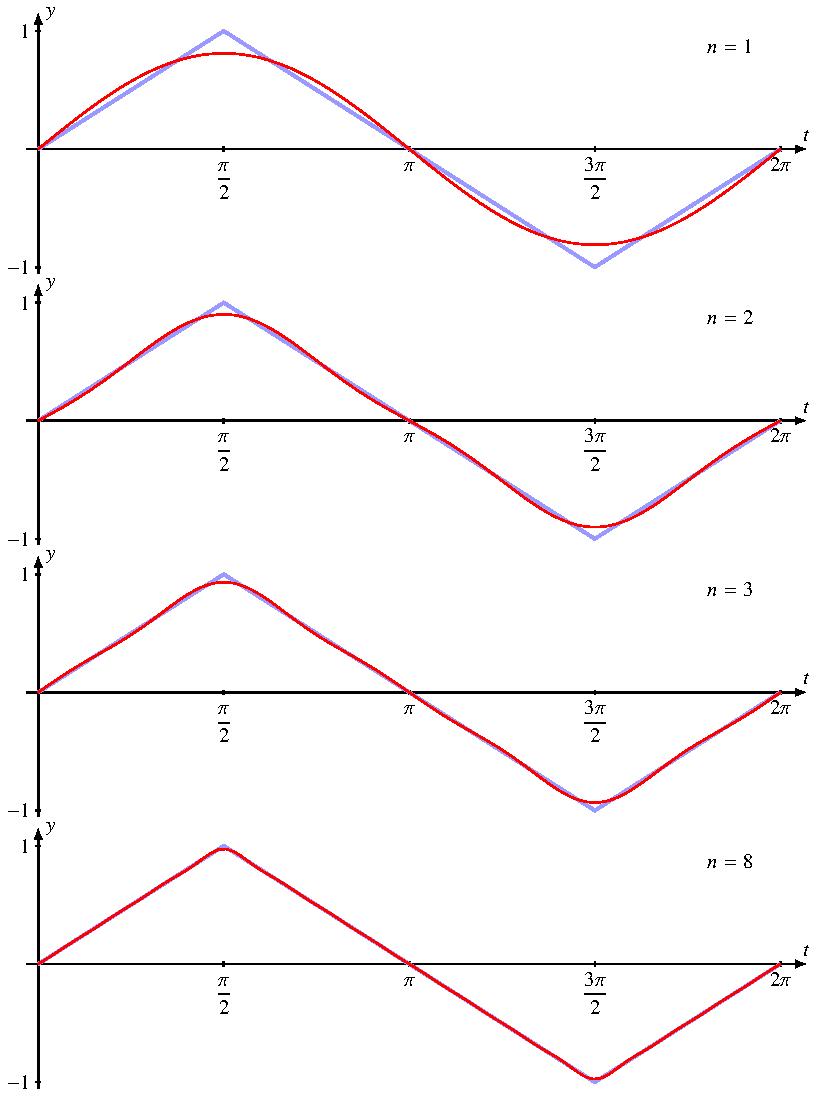
\includegraphics{chapters/6/dreieck2.pdf}
\caption{Dreiecksfunktion und Approximation durch die Fourierreihe
\eqref{skript:fourier:dreieckreihe}
für verschiedene Werte von $n$.
\label{skript:fourier:stetigdreieck}}
\end{figure}
Wir berechnen die Fourier-Koeffizienten für die Dreiecksfunktion
\eqref{skript:fourier:dreieck}, für die wir die diskreten Fourier-Koeffizienten
bereits in Abschnitt~\ref{subsection:fourier:dreiecksfunktion}
berechnet haben.
Wie im diskreten Fall folgt aus den Symmetrieeigenschaften, dass $a_k=0$
ist für alle $k$ und $b_k=0$ für alle geraden $k$.
Es bleibt also nur noch, für ungerades $k$
die Koeffizienten
\begin{align}
b_k
&=
\frac{1}{\pi} \int_0^{2\pi} f(x) \sin kx\,dx
\notag
\\
&=
\frac{4}{\pi} \int_{0}^{\frac{\pi}2} f(x)\sin kx\,dx
=
\frac{4}{\pi} \int_{0}^{\frac{\pi}2} \frac2{\pi}x\sin kx\,dx
=
\frac{8}{\pi^2} \int_{0}^{\frac{\pi}2} x\sin kx\,dx
\notag
\\
&=
\frac{8}{\pi^2} \biggl(
\biggl[-\frac{x}{k}\cos kx\biggr]_0^{\frac{\pi}2} + \int_{0}^{\frac{\pi}2}\frac{1}{k}\cos kx\,dx
\biggr)
=
\frac{8}{\pi^2}
\biggl[
-\frac{x}{k}\cos kx +\frac{1}{k^2}\sin kx
\biggr]_0^{\frac{\pi}2}
\notag
\\
&=
\frac{8}{\pi^2} \biggl[ \frac{\sin kx - kx\cos kx}{k^2}\biggr]_0^{\frac{\pi}2}
=
\frac{8}{\pi^2 k^2} \biggl[\sin kx - kx\cos kx\biggr]_0^{\frac{\pi}2}
\notag
\\
&=
\frac{8}{\pi^2k^2}\biggl(
(-1)^{(k-1)/2} - k\frac{\pi}2\underbrace{\cos k\frac{\pi}2}_{\displaystyle=0}
\biggr)
=
\frac{8}{\pi^2k^2}(-1)^{(k-1)/2}
\label{skript:fourier:bkstetig}
\end{align}
zu bestimmen.
In Tabelle~\ref{skript:fourier:beispiel} werden die diskreten
Fourierkoeffizienten den hier gefundenen stetigen Koeffizienten
gegenübergestellt.
Die zugehörige Fourierreihe
\begin{equation}
p_{2n}(t) = \frac{8}{\pi^2} \sum_{i=1}^n \frac{(-1)^i}{(2i-1)^2}\sin(2i-1)t
\label{skript:fourier:dreieckreihe}
\end{equation}
ist in Abbildung~\ref{skript:fourier:stetigdreieck} dargestellt.
Die Anzahl der berücksichtigten, nicht verschwindenden Terme ist $n$.

\subsection{Diskrete Fourier-Transformation}
Die Fourier-Koeffizienten $a_k$ und $b_k$ hängen linear von den
Funktionswerten $y_j$ ab.
Der Vektor der Fourier-Koeffizienten muss daher der Bildvektor des
Vektors $\vec y$ der Funktionswerte unter einer linearen Transformation
sein.
In diesem Abschnitt soll die diskrete Fourier-Transformation in etwas
mehr Detail hergeleitet werden.
Ausserdem soll gezeigt werden, wie die Fourier-Transformation
mit der schnellen Fouriertransformation
effizient berechnet werden kann, die in vielen Softwarepaketen zur
numerischen Berechnung implementiert ist.

\subsubsection{Transformationsmatrix}
Die Berechnung der Fourier-Koeffizienten ist eine lineare Operation
mit der $N\times N$-Matrix:
\[
A
=
\begin{pmatrix}
c_0^t\\
c_1^t\\
s_1^t\\
\vdots\\
c_{n-1}^t\\
s_{n-1}^t\\
c_n^t
\end{pmatrix}
=
\begin{pmatrix}
1           &1           &\dots &1            \\
\cos t_1    &\cos t_2    &\dots &\cos t_N     \\
\sin t_1    &\sin t_2    &\dots &\sin t_N     \\
\cos 2t_1   &\cos 2t_2   &\dots &\cos 2t_N    \\
\sin 2t_1   &\sin 2t_2   &\dots &\sin 2t_N    \\
\vdots      &\vdots      &\ddots&\vdots       \\
\sin(n-1)t_1&\sin(n-1)t_2&\dots &\sin(n-1)t_N \\
\cos nt_1   &\cos nt_2   &\dots &\cos nt_N    
\end{pmatrix}
\]
Die Orthogonalitätsrelationen von
Satz~\ref{skript:fourier:orthogonalitaet}
können jetzt neu geschrieben werden:
\begin{align*}
AA^t
&=
\begin{pmatrix}
c_0\cdot c_0&
	c_0\cdot c_1&
		c_0\cdot s_1&
			\dots&
				c_0\cdot c_{n-1}&
					c_0\cdot s_{n-1}&
						c_0\cdot c_n\\
c_1\cdot c_0&
	c_1\cdot c_1&
		c_1\cdot s_1&
			\dots&
				c_1\cdot c_{n-1}&
					c_1\cdot s_{n-1}&
						c_1\cdot c_n\\
s_1\cdot c_0&
	s_1\cdot c_1&
		s_1\cdot s_1&
			\dots&
				s_1\cdot c_{n-1}&
					s_1\cdot s_{n-1}&
						s_1\cdot c_n\\
\vdots	&\vdots	&\vdots	&\ddots	&\vdots	&\vdots	&\vdots	\\
c_{n-1}\cdot c_0&
	c_{n-1}\cdot c_1&
		c_{n-1}\cdot s_1&
			\dots&
				c_{n-1}\cdot c_{n-1}&
					c_{n-1}\cdot s_{n-1}&
						c_{n-1}\cdot c_n\\
s_{n-1}\cdot c_0&
	s_{n-1}\cdot c_1&
		s_{n-1}\cdot s_1&
			\dots&
				s_{n-1}\cdot c_{n-1}&
					s_{n-1}\cdot s_{n-1}&
						s_{n-1}\cdot c_n\\
c_n\cdot c_0&
	c_n\cdot c_1&
		c_n\cdot s_1&
			\dots&
				c_n\cdot c_{n-1}&
					c_n\cdot s_{n-1}&
						c_n\cdot c_n\\
\end{pmatrix}
\\
&=
\begin{pmatrix}
N     &0        &0        &\dots    &0        &0        &0        \\
0     &\frac{N}2&0        &\dots    &0        &0        &0        \\
0     &0        &\frac{N}2&\dots    &0        &0        &0        \\
\vdots&\vdots   &\vdots   &\ddots   &\vdots   &\vdots   &\vdots   \\
0     &0        &0        &\dots    &\frac{N}2&0        &0        \\
0     &0        &0        &\dots    &0        &\frac{N}2&0        \\
0     &0        &0        &\dots    &0        &0        &\frac{N}2
\end{pmatrix}.
\end{align*}
Bis auf die Faktoren $N$ und $\frac{N}2$ auf der Diagonalen ist
$AA^t$ 
eine Einheitsmatrix.
Wir können die Matrix zu einer Einheitsmatrix machen, indem wir 
$A$ mit der Diagonalmatrix
\begin{equation}
D
=
\begin{pmatrix}
\!\sqrt{\frac1N}&0&\dots&0\\
0&\!\sqrt{\frac{2}{N}}&\dots&0\\
\vdots&\vdots&\ddots&\vdots\\
0&0&\dots&\!\sqrt{\frac{2}{N}}
\end{pmatrix}
\end{equation}
multiplizieren.
Wir schreiben
\begin{align*}
{\cal F}
&=
D\, A
\end{align*}
Wir nennen $\cal F$ die {\em Fourier-Matrix}.
\index{Fourier-Matrix}%
Die Fourier-Matrix $\cal F$ ist orthogonal, es gilt
\[
{\cal F}{\cal F}^t
=
DAA^tD^t
=
DD^tAA^t
=
E,
\]
wobei wir im letzten Schritt $D^t$ mit $AA^t$ vertauschen durften,
weil beide Diagonalmatrizen sind.
Insbesondere erhält $\cal F$ das Skalarprodukt, womit wir natürlich
nur die Parseval-Identität anders formuliert haben.

%
% komplex.tex
%
% (c) 2018 Prof Dr Andreas Müller, Hochschule Rapperswil
%
\subsubsection{Komplexe Fouriertransformation}
Bisher wurden alle Rechnungen nur mit reellen Zahlen durchgeführt.
Es stellt sich aber heraus, dass komplexe Zahlen für die Beschreibung
der Fourier-Transformation sehr viel praktischer sind.
Der Grund dafür ist die Eulersche Beziehung
\[
e^{it} = \cos t + i \sin t.
\]
und die Rechenregel
\[
e^{a+b}=e^a\cdot e^b
\qquad\Rightarrow\qquad
e^{ikt}=\cos kt+i\sin kt
\]
für die Exponentialfunktion.
Für die Fourier-Koeffizienten werden die Summen
\[
a_0
=
\frac{1}{N}\sum_{j=1}^N y_j,\qquad
a_l
=
\frac{2}{N}\sum_{j=1}^N y_j \cos lt_j,
\qquad\text{und}\qquad
b_l
=
\frac{2}{N}\sum_{j=1}^N y_j \sin lt_j
\]
benötigt.
Fassen wir $a_l$ und $b_l$ als Real- und Imaginärteil einer komplexen
Zahl auf, dann können wir 
\begin{align*}
c_l
=
a_l+ib_l
&=
\frac2{N} \sum_{j=1}^N y_j (\cos lt_j + i \sin lt_j)
=
\frac2{N} \sum_{j=1}^N y_j e^{lt_j}
\end{align*}
berechnen.

Auch die Rekonstruktion~\eqref{skript:fourier:rekonstruktion} ist
mit komplexen Zahlen darstellbar.
Dazu verwendet man 
\[
\cos kt = \operatorname{Re} e^{ikt}
\qquad\text{und}\qquad
\sin kt = \operatorname{Im} e^{ikt}.
\]
In dieser Form
\[
f(t)
=
a_0
+\sum_{k=1}^n (a_k \cos kt + b_k \sin kt)
\]





%
% fft.tex -- Fast Fourier Transform
%
% (c) 2018 Prof Dr Andreas Müller, Hochschule Rapperswil
%
\subsubsection{Fast Fourier Transform}
\index{Fast Fourier Transform}
Die komplexe Darstellung der diskreten Fourier-Transformation ermöglicht
eine Formulierung, in der die Berechnung der Koeffizienten wie auch die
Auswertung des trigonometrischen Polynoms sehr viel schneller erfolgen
kann, wenigstens wenn $N$ gerade ist.
Die Bestimmung der $c_l$ verlangt die Berechnung der Produkte
$y_j e^{lt_j}$ für alle $j$ und $l$.
Ausserdem ist $t_j=2\pi j/N=lt_1$, die Exponentialfaktoren sind daher
$e^{lt_j}=(e^{t_1})^{lj}$.
Die Details dieses Algorithmus sollen hier nicht entwickelt werden,
es soll nur der Rechenaufwand abgeschätzt werden.
Die Anzahl der Multiplikationen dominiert die Laufzeit der Berechnung,
daher soll $g(N)$ die Anzahl der Multiplikationen für eine
Fourier-Transformation mit $N$ Termen bezeichnen.

Da $N$ gerade ist, kann man die Summe zur Berechnung der Koeffizienten
\begin{align}
c_l
&=
\sum_{j=0}^{N-1} y_j e^{-ilt_j}
\intertext{aufteilen in gerade und ungerade Terme}
&=
\sum_{j=0}^{N/2-1} y_{2j} e^{-ilt_{2j}}
+
\sum_{j=0}^{N/2-1} y_{2j+1} e^{-ilt_{2j+1}}
\notag
\\
&=
\sum_{j=0}^{N/2-1} y_{2j} e^{-ilj t_{2}}
+
e^{-ilt_1}
\sum_{j=0}^{N/2-1} y_{2j+1} e^{-ilj t_{2}}.
\label{skript:fft:split}
\end{align}
Es ist zu erkennen, dass jeder Summand eine Fourier-Transformation
mit der halben Anzahl von Datenpunkten und der doppelten Schrittweite
$t_2$ statt $t_1$ ist.
Schreiben wir 
\[
\begin{aligned}
y'_j
&= 
y_{2j}&j&=0,\dots,\frac{N}2
\\
y''_j
&=
y_{2j+1}&j&=0,\dots,\frac{N}2
\end{aligned}
\]
für die geraden bzw.~ungeraden Elemente, dann ist er erste Summand in
\eqref{skript:fft:split} die Fouriertransformation von $y'$, der zweite
Summand enthält die Fouriertransformation von $y''$, es ist also
\[
c_l = c'_l + e^{-ilt_1} c''_l.
\]
Der zusätzliche Aufwand für die Berechnung von $c_l$ aus $c'_l$ und $c''_l$
ist also nur gerade eine Multiplikation mit einem Exponentialfaktor.

Der Aufwand für die Berechnung der Koeffizienten $c_l$ setzt sich also
zusammen aus dem Aufwand für zwei Fourier-Transformationen mit Länge $N/2$
und $N$ Multiplikationen, eine für jeden der Koeffizienten $c_l$.
Dies führt auf die Rekursionsformel
\begin{equation}
g(N) = 2g(N/2) + N.
\label{skript:fft:rekursion}
\end{equation}
Wenn $N=2^m$ sogar eine Zweierpotenz ist, dann lässt sich diese
Idee iterieren und damit $g(2^m)$ iterativ aus $g(2)$ berechnen.

Die Rekursionsformel
\eqref{skript:fft:rekursion}
hat die Lösung $g(N) = N\log_2 N$, wie man durch Einsetzen in die
rechte Seite von
\eqref{skript:fft:rekursion}
prüfen kann:
\[
2g(N/2) + N
=
2\cdot\frac{N}2\log_2\frac{N}2 + N
=
N(\log_2 N - 1) + N
=
N\log_2 N
=
g(N).
\]
Wir schliessen daraus, dass der Aufwand für die Berechnung der
Fourier-Transformation mit diesem Algorithmus von der Grössenordnung
$O(N\log N)$ ist, also deutlich schneller als die naive Berechnung
mit der Summenformel, die Aufwand $O(N^2)$ verlangt.
\begin{figure}
\centering
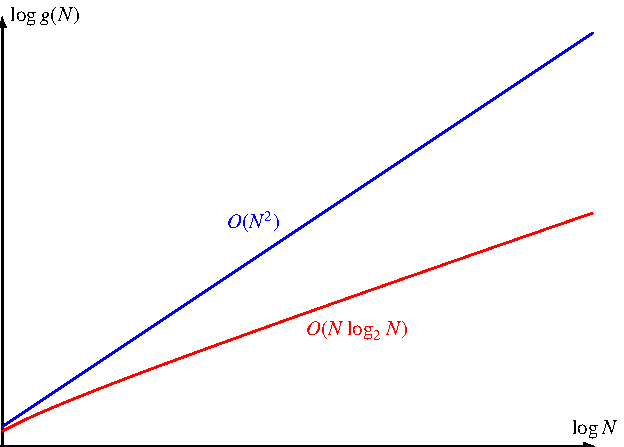
\includegraphics{chapters/6/fftaufwand.pdf}
\caption{Aufwand für die komplexe Fouriertransformation ({\color{blue}blau})
im Vergleich mit
dem Aufwand für die schnelle Fourier-Transformation ({\color{red}rot}).
\label{skript:fft:aufwandgraph}}
\end{figure}
In Abbildung~\ref{skript:fft:aufwandgraph} sind die beiden Aufandkurven im 
Vergleich dargestellt.

Diese schnelle Variante der Fourier-Transformation wurde von Cooley 
\index{Cooley, J.~W.}%
und Tukey 1965 veröffentlicht.
\index{Tukey, J.~T.}%
Das Verfahren war allerdings auch schon Carl Friedrich Gauss bekannt,
\index{Gauss, Carl Friedrich}
er hat es zur Berechnung der Bahnelemente der Asteroiden Pallas und
Juno verwendet.
Der Algorithmus wird von vielen Softwarepaketen für numerische Berechnung
implementiert.
Sehr verbreitet ist die Bibliothek FFTW3 (Fastest Fourier Transform in the
West, Version 3) \cite{skript:fftw}. 
Diese Bibliothek wird zum Beispiel auch von Octave verwendet um die
Funktion \texttt{fft} zu implementieren.
\index{fft@\texttt{fft}}%
Sie ist sehr einfach zu verwenden: als Argument wird der Vektor der
$y$-Werte übergeben, der Rückgabewert ist der Vektor der komplexen
Koeffizienten $c_l$.
Der Koeffizient $c_0$ ist das erste Element im Rückgabevektor, gefolgt
von $c_1,\dots,c_{N/2-1}$.
Der Koeffizient $c_{-1}$ ist das letzte Element im Rückgabevektor, davor
steht $c_{-2}$.
Als Zeilenvektor geschrieben ist der Rückgabewert von \texttt{fft}
\[
( c_0, c_1, c_2, \dots , c_{n-1}, c_n=c_{-n},
c_{-n+1},c_{-n+2},\dots, c_{-2},c_{-1}).
\]


%Für reelle Werte $y_j$ haben die Koeffizienten $c_l$ zusätzliche
%Symmetrieeigenschaften.
%Die komplex konjugierte $\bar c_l$ ist
%\[
%\bar c_l
%=
%\overline{\sum_{j=0}^{N-1} y_j e^{2\pi ijl/N}}
%=
%\sum_{j=0}^{N-1} y_j e^{-2\pi i jl/N}
%=
%c_{-l}.
%\]
%Daraus liest man zum Beispiel ab, dass $c_0\in\mathbb R$ ist, nämlich
%\[
%c_0 = \frac{1}{N} \sum_{j=0}^{N-1} y_j = a_0.
%\]
%Für die anderen Koeffizienten gilt zunächst
%\begin{align*}
%c_l
%&=
%\frac{1}{N}\sum_{j=0}^{N-1} y_j e^{-2\pi ilj/N}
%=
%\frac{1}{N}\sum_{j=0}^{N-1} y_j \biggl(\cos \frac{2\pi lj}{N} + i \sin\frac{2\pi lj}{N}\biggr)
%\\
%&=
%\frac{1}{N}\sum_{j=0}^{N-1} y_j
%\cos \frac{2\pi lj}{N}
%+
%i
%\frac{1}{N}\sum_{j=0}^{N-1} y_j
%\sin\frac{2\pi lj}{N}
%\\
%&=
%\frac12(a_l + ib_l)
%\end{align*}
%Zusammen mit der Beziehung $\bar c_l=c_{-l}$, können wir die reellen
%Fourier-Koeffizienten auch verwenden, um die reellen Koeffizienten
%\begin{align*}
%a_l
%&=
%c_l + c_{-l}
%&&\text{und}&
%b_l
%&=
%\frac1{i}
%(c_l - c_{-l})
%\end{align*}
%durch die komplexen Koeffizienten auszudrücken.

In der Übungsaufgabe zu diesem Kapitel wird verlangt die
Fourier-Koeffizienten von Hand zu berechnen.
Mit der Funktion \texttt{fft} in Octave kann dies jetzt natürlich viel
schneller erreicht werden.
Wendet man \texttt{fft} auf den Vektor
\[
y = (-3.2, -13.6, -12.3, -3.9, 3.1, 2.0, -4.1, -6.1, 0.5, 10.7, 16.3, 10.6 )
\]
erhält man einen Vektor mit 12 komplexen Fourier-Koeffizienten.
Wie im letzten Abschnitt erklärt, können wir die reellen Fourier-Koeffizienten
$a_k$ und $b_k$ wieder erkennen.
Man liest ab:
\[
\texttt{fft}(y) / 6
=
\left[
\begin{tabular}{>{\tt}r}
   0.00000 + 0.00000i\\
   0.34210 + 7.52778i\\
  -3.57500 + 9.16544i\\
   0.08333 + 0.25000i\\
  -0.12500 + 0.15877i\\
   0.02456 + 0.02222i\\
   0.10000 + 0.00000i\\
   0.02456 - 0.02222i\\
  -0.12500 - 0.15877i\\
   0.08333 - 0.25000i\\
  -3.57500 - 9.16544i\\
   0.34210 - 7.52778i
\end{tabular}
\right]
\qquad\Rightarrow\qquad
\begin{tabular}{|>{$}c<{$}|>{$}r<{$}|>{$}r<{$}|}
\hline
k     &\hat{a}_k&\hat{b}_k\\
\hline
0     & 0.00000&        \\
1     & 0.34210&-7.52778\\
2     &-3.57500&-9.16544\\
3     & 0.08333&-0.25000\\
4     &-0.12500&-0.15877\\
5     & 0.02456&-0.02222\\
6     & 0.10000&        \\
\hline
\end{tabular}
\]
Die direkte Berechnung in der Aufgabe~1 führt auf die gleichen Werte.





